%
% General structure for the revdetua class:
%
\documentclass[portugues,final]{revdetua}
\usepackage[portuguese]{babel}
\usepackage{listingsutf8}
\usepackage[utf8]{inputenc}
\usepackage[T1]{fontenc}
\usepackage{graphicx}
\usepackage{hyperref}
\usepackage{wrapfig}
\usepackage{float}
\usepackage{color}
\usepackage{eurosym}
%
% Valid options are:
%
%   longpaper --------- \part and \tableofcontents defined
%   shortpaper -------- \part and \tableofcontents not defined (default)
%
%   english ----------- main language is English (default)
%   portugues --------- main language is Portuguese
%
%   draft ------------- draft version
%   final ------------- final version (default)
%
%   times ------------- use times (postscript) fonts for text
%
%   mirror ------------ prints a mirror image of the paper (with dvips)
%
%   visiblelabels ----- \SL, \SN, \SP, \EL, \EN, etc. defined
%   invisiblelabels --- \SL, \SN, \SP, \EL, \EN, etc. not defined (default)
%
% Note: the final version should use the times fonts
% Note: the really final version should also use the mirror option
%

\begin{document}

% Note: the month must be in Portuguese

\title{\textbf{Jogo de Xadrez implementado em OpenGL} \\ Computação Visual\\Universidade de Aveiro}
\author{Diogo Silva 60337}
\maketitle
\begin{resumo} % Note: in Portuguese
Este relatório descreve detalhadamente a estrutura e o motor de jogo de Xadrez implementado em OpenGL.
Relatório inclui descrição de shaders, modelos, skybox, texturas, iluminação, movimentos, entre outras situações.
\end{resumo}

%\begin{palavraschave} % Note: in Portuguese (optional)
%\end{palavraschave}

\section{Estrutura da Aplicação}

A aplicação do jogo inicialmente encontrava-se em C, tal como foi sugerido nas aulas, mas devido à necessidade de introduzir o conceito de herança nas peças de Xadrez, passou-se tudo para {\tt C++} e realizou-se o desenvolvimento a partir daí.\\

Para compilar o código foi criado um tutorial num ficheiro {\tt README} com uma explicação breve a dizer as bibliotecas que são necessárias instalar e de como correr o programa.

\subsection{Engine do Jogo de Xadrez}

O motor do jogo tem as seguintes funcionalidades como:
\begin{enumerate}
\item{Obter lista das referências para cada peça}
\item{Verificar se o jogo já acabou e quem ganhou}
\item{Verificar de quem é a vez de jogar}
\item{Realizar um movimento}
\item{Mostrar movimentos possíveis de uma peça}
\end{enumerate}

Tal como mostra a figura seguinte, pode-se verificar que estas funcionalidades são acedidas facilmente através da classe Chess.

\begin{figure}[H]
\centerline{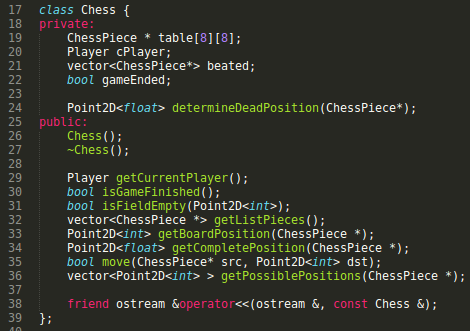
\includegraphics[width=230pt]{images/chess.png}}
\caption{Implementação do Chess}
\label{img:complete}
\end{figure}

Por sua vez, a classe Chess contém uma matrix de 8 por 8 (64 lugares) em que no ínicio, estão 32 ocupadas e as restantes apontar para {\tt NULL}, esta matrix é uma matrix de referências de Peças de Xadrez, mais precisamento, objectos do tipo ChessPiece (descritos detalhadamente na secção seguinte).

\subsubsection{Peças do Xadrez}

As peças de Xadrez têm um módulo do qual permite destinguir a qual jogador pertence a peça, o tipo da peça (se é um Rei, um Cavalo, etc..). Consecutivamente, também é o que permite destinguir movimentos das peças.\\

Todas as peças herdam uma classe principal chamada ChessPiece, que contém as funcionalidades referidas anteriomente, tal como mostra a figura seguinte:

\begin{figure}[H]
\centerline{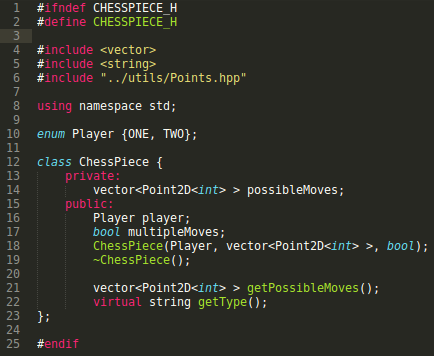
\includegraphics[width=230pt]{images/chesspiece.png}}
\caption{Implementação do ChessPiece}
\label{img:complete}
\end{figure}

Tal como foi referido, todas as peças têm de indicar na sua inicialização a lista de movimentos possíveis, se são movimentos multíplos ou não e o jogador a qual pertence, na figura seguinte pode-se ver o exemplo da implementação da Rainha, em que mostra que os movimentos possíveis são em todas as casas as sua volta e são movimentos multíplos.

\begin{figure}[H]
\centerline{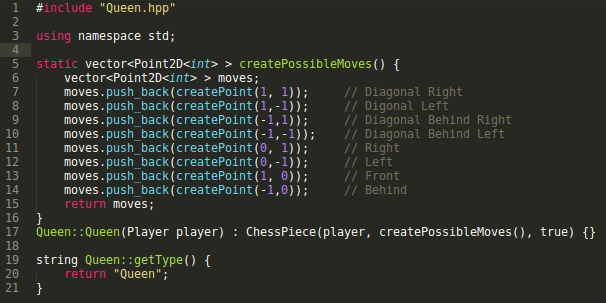
\includegraphics[width=230pt]{images/queen.png}}
\caption{Implementação da Peça Rainha}
\label{img:complete}
\end{figure}

\subsection{Desenvolvimento OpenGL}

Relativamente a implementação da parte gráfica da aplicação, decidiu-se dar continuação a estrutura já existentes das aulas, tendo os seguintes ficheiros:
\begin{enumerate}
\item{{\tt init.cpp}, que inicia todos os modelos, fontes de luz, estruturas, janela e callbacks}
\item{{\tt models.cpp}, que permite ler os ficheiros obj do formato oficial}
\item{{\tt globals.cpp}, contém algumas variaveis globais para permitir fácil manipulação durante o uso de callbacks}
\item{{\tt callbacks.cpp}, este ficheiro é o que trata de reescrever a imagem, trata também ainda dos movimentos do rato e cliques do teclado}
\item{{\tt shaders.cpp}, este ficheiro é o que carrega o vertex e o fragment shader}
\end{enumerate}

Para além deste ainda foram criados dois ficheiros, um {\tt LightModel.cpp} que contém apenas todas as caracteristicas necessárias para a representação de um foco de iluminação, tais como, posição do foco, intensidade do foco e intensidade da luz ambiente.
O outro ficheiro, é o ficheiro {\tt GraphicModelChess.cpp} que contém as caracteristicas gráficas de cada modelo de Xadrez (este ficheiro é descrito detalhamente na secção seguinte).

\subsubsection{Modelos}

{\large Estrutura do GraphicModelChess}

A classe GraphicModelChess contém todas as caracteristicas gráficas de cada modelo:
\begin{enumerate}
\item{Número de vertíces}
\item{Lista de vertíces}
\item{Lista das normais}
\item{Valores de deslocamento, rotação e de redimensionamento}
\item{Coeficiente Ambiente, Difusão, Especular e Phong}
\end{enumerate}

Para além deste valores, ainda contém uma referência para o respectivo modelo de Xadrez, ou seja, objecto ChessPiece.

A figura seguinte mostra o cabeçalho deste ficheiro:

\begin{figure}[H]
\centerline{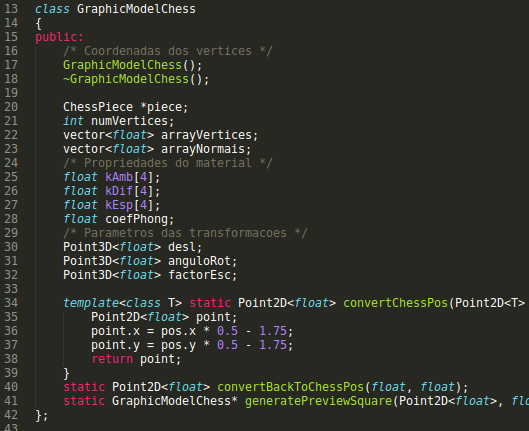
\includegraphics[width=230pt]{images/graphicmodelchess.png}}
\caption{Cabeçalho do GraphicModelChess}
\label{img:complete}
\end{figure}

Ainda se pode verificar a existência de 3 funções estáticas, duas das quais servem para converter coordenadas do tabuleiro de Xadrez para coordenadas do mundo 3D, e vice-versa. A outra função serve para gerar modelos quadrados que vão servir para representar todas as alternativas possíveis de cada movimento.\\

{\large Load de cada modelo de Xadrez}\\

As peças do Xadrez foram retiradas de modelos já existentes num projecto Open Source \cite{pwag}, desse projecto foram retirados do directório /trunk/Chess/Chess/Models.\\

Sendo que esses modelos foram todos optimizados usando o programa Blender de maneira a ficarem da forma pretendida, tal como, colocar a base no plano xOy, ou seja, z = 0.

Após a recolocação dos modelos, foram todos exportados para ficheiros .obj no formato oficial.

Apesar de fazer a leitura do modelo oficial dos ficheiros obj, apenas são carregados os vertices, as normais e as faces, deixando de foram os vertices das texturas.

O load genérico dos ficheiros obj encontra-se em {\tt /src/models.cpp}.

\subsubsection{Shaders}

Inicialmente os shaders apenas estavam a ser usados para a representação das cores, não fazendo qualquer procesamento na gráfica, mas houve a necessidade de implementar a iluminação nos shaders devido ao tentar fazer uma animação mais complexa e notar-se que a imagem não era completamente fluída porque o tempo que o CPU demorava a fazer os calculos das iluminações de cada vertice era superior ao tempo da rotação, verificando-se um delay no movimento.\\

Sendo assim, havia duas opções, tornar a animação mais rudimentar, ou passar a iluminação para os shaders (fazendo com que a gráfica processa-se a animação).

\begin{figure}[H]
\centerline{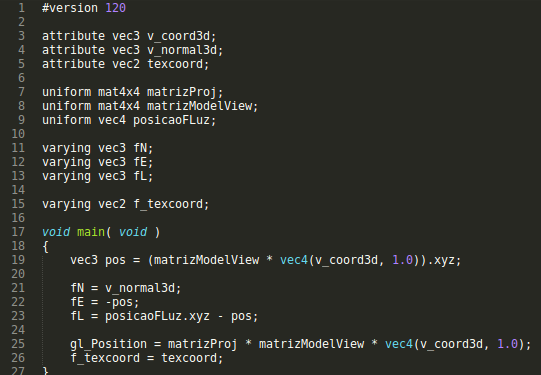
\includegraphics[width=230pt]{images/vertexshader.png}}
\caption{Vertex Shader}
\label{img:complete}
\end{figure}

Como se pode verificar no vertex shader é feito os calculos do ponto relativamente a um vertice, a sua posição, consoante a matrix projecção e o modelo, para além disso, ainda é calculado alguma fracções que vão ser usadas mais tarde pelo fragment shader, estas precisam de ser calculadas no vertex porque a iluminação depende da posição do vertice e do foco de iluminação.\\

Ainda se pode verificar que as coordenadas das texturas são passadas para o fragment shader.

\begin{figure}[H]
\centerline{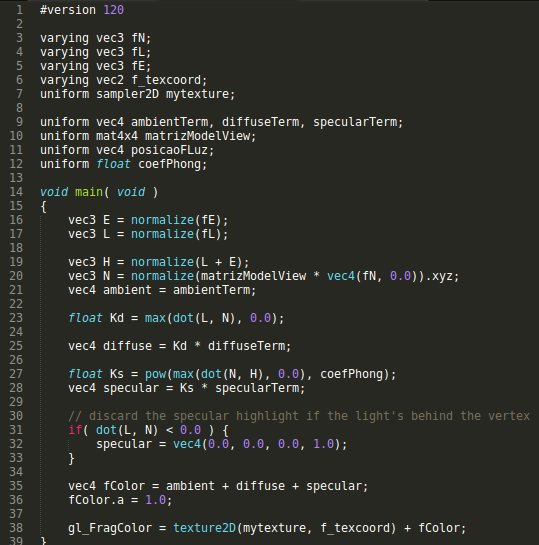
\includegraphics[width=230pt]{images/fragmentshader.png}}
\caption{Fragment Shader}
\label{img:complete}
\end{figure}

No fragment shader pode-se verificar que são usadas as variaveis passadas pelo Vertex Shader, neste caso, fE, fN e fL, calculando a respectiva cor do vertice, dando o efeito de iluminação pretendido.\\

Para realizar esta parte do código foi utilizado os slides dados na teórica das aulas de Computação Visual no ficheiro PDF ``Métodos de Iluminação e Sombreamento (PDF)''\cite{shadingAulas} nos slides 50 a 53 e ainda foi consultado wikibooks relativamente a OpenGL para conciliar iluminação e texturas\cite{lightningsurfaces}.\\

Ainda se pode verificar que as texturas são introduzidas\cite{textures} com o texture2D que permite aplicar uma cor RGB a uma coordenada específica, fazendo isto com todas as coordendas, para além disto, ainda se pode verificar que dá-se igual importância a textura e a iluminação, apesar de não ser o melhor método funciona relativamente bem.

\section{Aspectos Importantes do Trabalho}

Os aspectos importantes deste trabalho vai desde a representação gráfica dos objectos (como peças de xadrez, texturas, skybox, movimentos possíveis de cada peça) e interacção com o utilizador (como clique nas peças de xadrez, teclado ou rato, e ainda manipulação da cena, teclado ou rato).

\subsection{Interacção com o utilizador}

\subsubsection{Clique nas peças do Xadrez (Interacção Directa)}

Para permitir o clique nas peças do Xadrez através do rato foi necessário pegar nas coordenadas X, Y do clique do rato e converter para o mundo 3D, para além disso, ainda foi necessário calcular a profundidade do pixel respectivo\cite{objectsel}.

Para calcular a profundidado do pixel respectivo, ou seja, do eixo Z, usou-se a função de OpenGL glReadPixels na qual se obteve a coordenada Z do respectivo pixel ( {\tt glReadPixels(x, int(winY), 1, 1, GL\_DEPTH\_COMPONENT, GL\_FLOAT, \&winZ)} ) e depois a partir das 3 coordenadas usou-se a função de OpenGL gluUnProject passando por argumento, as coordenadas 3D do clique, a matriz projecção e a dimensão do viewport, recebendo por referência o valor do ponto 3D nas coordenadas reais, podendo assim verificar onde é que o utilizar carrega, ou seja, em que local do tabuleiro carregou.

\begin{figure}[H]
\centerline{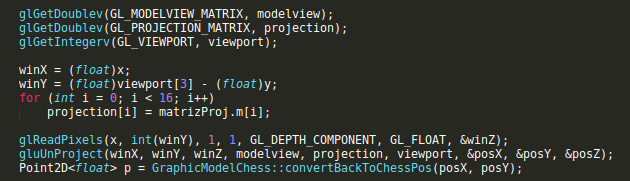
\includegraphics[width=230pt]{images/unproject.png}}
\caption{Conversão de Viewport para Posição do Mundo 3D}
\label{img:complete}
\end{figure}

Para além do clique das peças também a possível intercalar entre cada peça usando a tecla + ou -
Para alterar entre as posições possíveis da peça seleccionada usa-se a tecla . ou ,
E ainda a tecla ``m'' para fazer a peça mover-se para a posição seleccionada.

\subsubsection{Manipulação do cenário}

A manipulação do cenário é possível através de rato e teclado, sendo que com o rato é possível visualizar o tabuleiro de qualquer ângulo, enquanto que com o teclado só roda sobre o eixo do Z, ou seja, a volta do tabuleiro.

Para fazer a manipulação do cenário com o rato, foi usada a callback glutMotionFunc(onDrag) que permite detectar movimentos contínuos do rato (cliques sem largar o botão), calculando a diferença com a posição anterior do ângulo e fazendo rodar essa diferença.

Também é possível aumentar ou diminuir a cena (efeito de zoom) usando o scroll do rato.

\subsection{Iluminação na Placa Gráfica}

Como foi referido anteriormente, na secção da estrutura dos Shaders, houve a necessidade de passar a iluminação do CPU para a placa gráfica devido ao processamento das animações estar muito lento.

Como se pode verificar na imagem seguinte, o foco de iluminação está colocado na posição x = 0 e y = 0, com uma intensidade média, apenas para provocar uma luz ambiente no centro do tabuleiro, ainda se pode verificar a reflexão da iluminação em cada peça do Xadrez apontar para o centro.

\begin{figure}[H]
\centerline{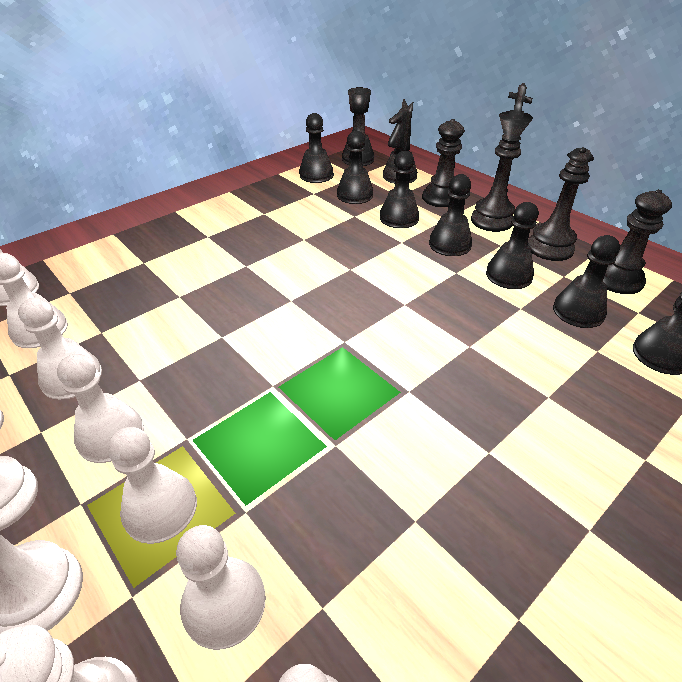
\includegraphics[width=230pt]{images/illumination.png}}
\caption{Iluminação do Tabuleiro}
\label{img:complete}
\end{figure}

\subsection{Texturas}

Foram aplicadas duas texturas distintas, textura do tabuleiro, que inclui o quadriculado do Xadrez e a respectiva cor.
Outra solução que podia ter sido aplicada era criar 64 planos (32 brancos e 32 pretos) a simular o tabuleiro de Xadrez, mas tendo em conta que é mais realista aplicar uma textura, optou-se por essa solução, sendo que a textura aplicada foi a seguinte:

\begin{figure}[H]
\centerline{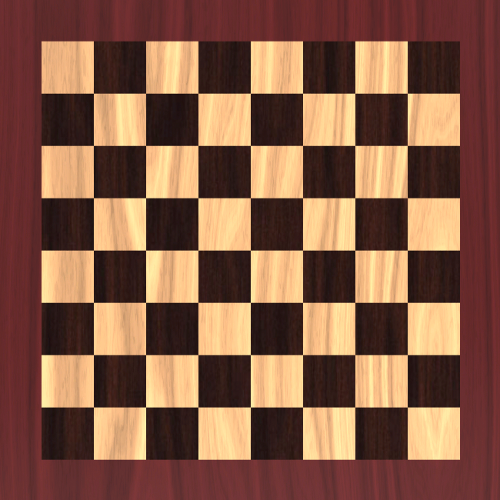
\includegraphics[width=150pt]{images/chessboard.png}}
\caption{Textura do Tabuleiro de Xadrez}
\label{img:complete}
\end{figure}

E para além disso ainda foi usada uma textura a simular a madeira, em que as peças do Xadrez podem usar madeira mais escura (perto de preto) ou madeira mais clara (perto de branco), conseguindo assim fazer a distinção das peças do jogador um e do jogador dois, sendo que o jogador um usa as peças com a textura branca e o jogador dois usa as peças com a textura preta. Como se pode ver na imagem seguinte o exemplo para as peças do jogador dois:

\begin{figure}[H]
\centerline{
\includegraphics[width=150pt]{images/basic_black.png}}
\caption{Textura das peças do jogador 2}
\label{img:complete}
\end{figure}

O detalhe sobre como as texturas são carregadas é referido anteriormente no relatório na parte referente a estrutura do código em Shaders.

\subsection{Skybox}

A skybox é o conceito de criar um ambiente de fundo que simule o mundo 3D, como por exemplo, o céu, se colocar uma imagem simples do céu como fundo não vai dar a perspectiva 3D, porque se o utilizador rodar o ambiente a imagem vai se manter estática, então surgiu o conceito de Skybox que é um cubo em que as suas texturas são uma imagem completa da visão do céu a 360º, conseguindo assim dar a perspectiva que o céu também muda se mudarmos a câmera.

A imagem utilizada foi a seguinte:

\begin{figure}[H]
\centerline{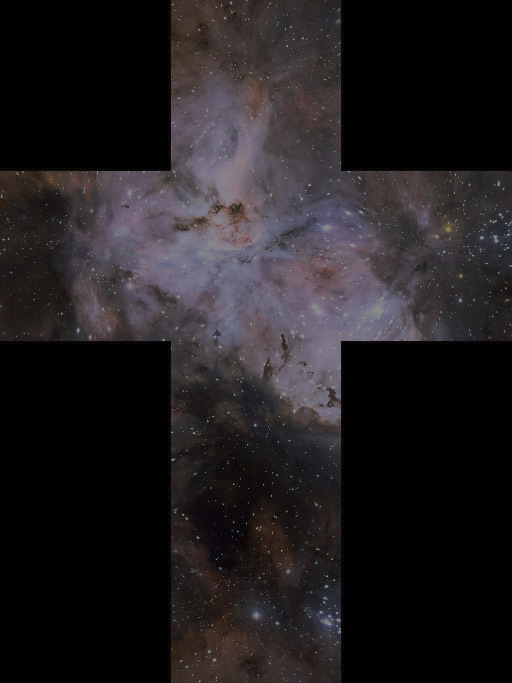
\includegraphics[width=150pt]{images/skybox.png}}
\caption{Textura utilizada para a Skybox}
\label{img:complete}
\end{figure}

Sendo que esta imagem foi aplicada (através de texturas) a um cubo com dimensões superior ao tabuleiro e modificando a cor, mudando o coeficiente ambiente para (0.5, 0.8, 1) RGB, ou seja, uma espécie azul claro para simular o céu.

Se verificarmos a skybox de fora, é possível verificar que é apenas um cubo com texturas.

\begin{figure}[H]
\centerline{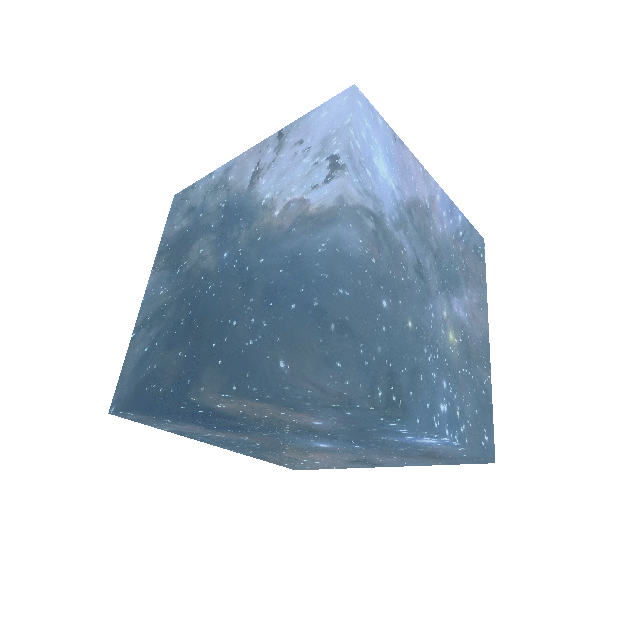
\includegraphics[width=230pt]{images/skybox_cube.png}}
\caption{Textura utilizada para a Skybox}
\label{img:complete}
\end{figure}

Apesar que por defeito, não é permitido fazer zoom para fora da skybox, mas alterando o código nas callbacks pode ser possível.

\subsection{Representação Gráfica}

\subsubsection{Movimentos possíveis das peças}

Na imagem seguinte pode-se verificar que é possível ver todas movimentações possíveis de cada peça de Xadrez:

\begin{figure}[H]
\centerline{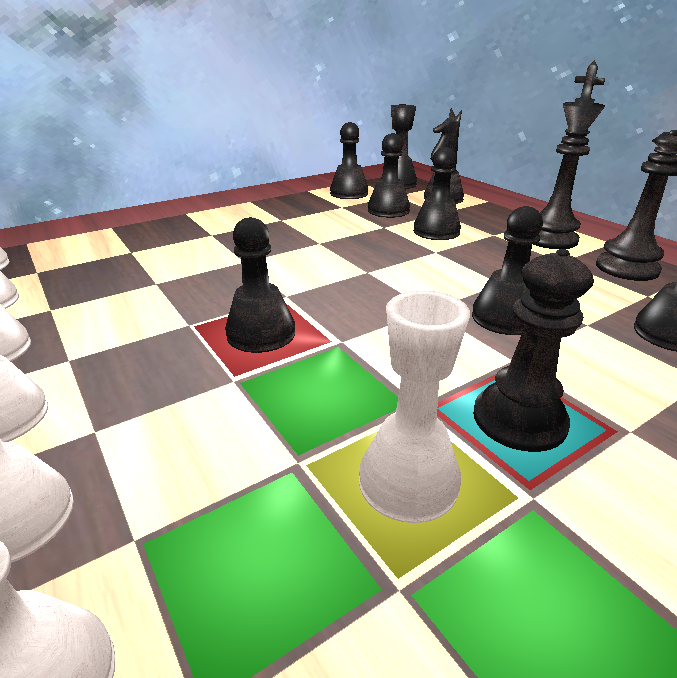
\includegraphics[width=230pt]{images/towerkill.png}}
\caption{Torre branca seleccionada}
\label{img:complete}
\end{figure}

Nesta imagem é possível verificar que a torre branca é a peça seleccionada (casa amarela) e que pode matar a rainha preta ou o peão preto (casas vermelhas), mas também pode avançar para as casas verdes sem matar nenhuma das peças inimigas. Ainda é possível verificar que a torre tem a casa da rainha preta seleccionada.

A previsão dos movimentos são simples planos 2D, com dois triângulos para formar um quadrado proporcional a quadrícula do tabuleiro.\\

{\large Distinção das casas de movimentos}\\

A distinção dos movimentos existentes foi feita através de cores, sendo que a casa que está amarelo pertence a casa da peça que está seleccionada, as casas que estão a verde são aquelas para as quais a peça se pode movimentar sem matar nenhuma peça inimiga e as casas vermelhas são aquelas em que a peça pode-se movimentar matando a peça inimiga. Ainda temos a casa azul, que representa a casa para a qual a peça se vai mover, mais precisamente, a casa que está seleccionada.

\subsubsection{Peças mortas}

Para representar as peças quando morrem pensou-se na situação real, quando um jogador mata a peça do adversário por norma costuma-se colocar essa peça ao pé de si, neste caso, optou-se por colocar a peça do lado direito do tabuleiro em fila (a medida que vai matando as peças adversárias). 

Para fazer este efeito apenas teve de ser efectuado uma translação sobre a peça que morre.

\section{Resultado Final}

O resultado final obtido foi o seguinte:

\begin{figure}[H]
\centerline{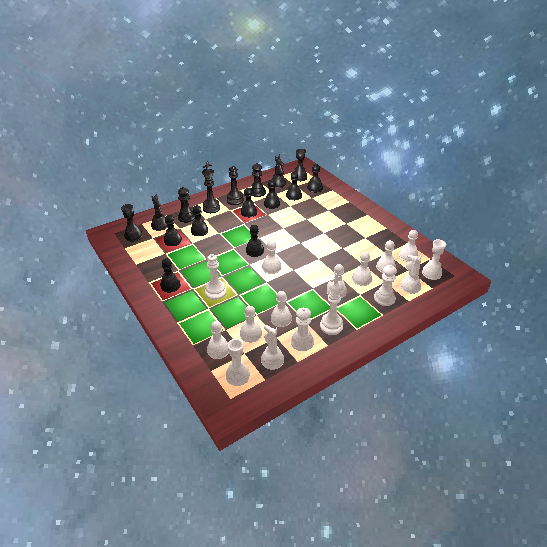
\includegraphics[width=230pt]{images/sample.png}}
\caption{Resultado final}
\label{img:complete}
\end{figure}

Pode-se verificar que OpenGL apesar de não ser uma biblioteca de muito alto nível, é possível fazer a representação gráfica de objectos bastante complexos usando apenas triângulos. Neste trabalho foi possível realizar texturas, skybox, leitura de ficheiros obj, iluminação na placa gráfica, motor do jogo e interecção com o utilizador (rato e teclado).

\section{Compilação e Execução}

Código fonte disponível em:

{\tt \url{https://github.com/dbtds/chess-opengl}}

Podendo ser obtido através do comando: {\tt git clone https://github.com/dbtds/chess-opengl.git}

Este projecto foi desenvolvido unicamente em ambiente Linux, sendo assim, não foi criado qualquer ficheiro executável para ambiente Windows, apesar que também é possível faze-lo alterando apenas a forma de compilação.\\

Note-se que todas as próximas indicações foram apenas realizadas em ambiente Linux no Ubuntu 14.10 64 bits.\\

Software essencial para compilar e correr o programa:
\begin{enumerate}
\item build-essential
\item qt4-qmake
\item libglew-dev
\item freeglut3-dev
\end{enumerate}

Para obter cada dependência basta executar:

{\tt sudo apt-get install dependency\_name}

Após a obtenção de todas estas dependências, basta executar o Makefile na pasta principal (root).

Executando em bash {\tt / \$ make}

Para executar o programa, basta ir a pasta gerada bin, e correr o executável com o nome chess.
Executando em bash {\tt /bin \$ ./chess}

Já existe um executável pré-gerado apenas para 64 bits dentro da pasta bin com o nome chess\_bin64, executando da mesma forma:
Em bash {\tt /bin \$ ./chess\_bin64}


\bibliography{report} % use a field named url or \url{} for URLs
%\url{www.ua.pt}
% Note: the \bibliographystyle is set automatically

\end{document}
